\documentclass{standalone}
\usepackage{tikz}
\usetikzlibrary{angles, quotes}

\begin{document}


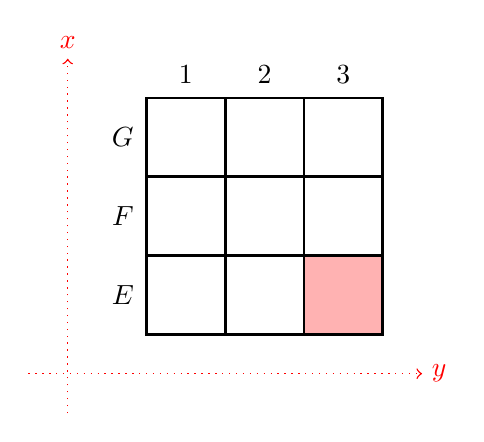
\begin{tikzpicture}[line width=1pt]

   	\fill[red!30] (2,0) rectangle (3,1);
    \draw (0,0) rectangle (3,3);
    \draw (0,1) -- (3,1) coordinate (A);
    \draw (0,2) -- (3,2) coordinate (A2);
    \draw (1,0) -- (1,3) coordinate (A3);
    \draw (2,0) -- (2,3) coordinate (A4);

    \node at (-.3,.5) {$E$};
    \node at (-.3,1.5) {$F$};
    \node at (-.3,2.5) {$G$};
    \node at (.5,3.3) {$1$};
    \node at (1.5,3.3) {$2$};
    \node at (2.5,3.3) {$3$};

    \draw[line width=0.5pt,->,red, dotted] (-1.5,-.5) -- (3.5,-.5) node[right] {$y$};
    \draw[line width=0.5pt,->,red, dotted] (-1,-1) -- (-1,3.5) node[above] {$x$};

\end{tikzpicture}
 	
\end{document}
